\chapter{\IfLanguageName{dutch}{Evaluatieproces}{Evaluationproces}}%
\label{ch:evaluatieproces}
\section{Inleiding}
Het interpreteren van gevoelens en boodschappen uit kunstwerken is een zeer persoonlijk iets. Het beoordelen van de effectiviteit van de applicatie is dus een uitdagende taak zijn. Om een grondige evaluatie van onze kunstwerken mogelijk te maken, hebben we besloten om een Turingtest te implementeren als onderdeel van ons evaluatieproces. Hierbij zullen we werken met een diverse set persona's, waaronder deelnemers van verschillende geslachten, leeftijden, hobbies en artistieke achtergronden. Bovendien zullen we een onderscheid maken tussen persona's die het nieuws volgen en degenen die dat niet doen. \\

Het doel van ons evaluatieproces is om de interpretatie en relevantie van de kunstwerken te valideren. Het resultaat van de turingtest kun je vinden in punt \ref{section:result}
\section{Turingtest}
 Door deelnemers te vragen specifiek nieuws te identificeren dat zij associëren met elk schilderij, kunnen we hun begrip van de context en hun vermogen om de artistieke interpretatie te verbinden met actuele gebeurtenissen beoordelen. We zullen de deelnemers vragen om specifieke nieuwsgebeurtenissen te identificeren die zij associëren met elk schilderij. Dit stelt ons in staat om hun begrip van de context te beoordelen en te zien of ze in staat zijn om de artistieke interpretatie van het schilderij te verbinden met actuele gebeurtenissen. Indien een deelnemer een onjuiste associatie maakt, zullen we het betreffende nieuwsartikel tonen en vervolgens vragen of ze het nieuwsgebeuren herkennen.. Indien een deelnemer geen nieuws volgt, kunnen we hem altijd vragen te gokken naar wat er zou kunnen ge-associeerd zijn met deze kunstwerk om te weten welk gevoel of boodschap dit overbrengt. \\
 
 In deze test zullen we deelnemers vragen om drie verschillende schilderijen te bekijken, elk verkregen door de de applicatie van de laatste drie dagen. De taak van de deelnemers is om aan te geven welk nieuwsgebeuren zij herkennen in elk van de schilderijen.
  
\section{Persona}
Zoals eerder vermeld zullen we tijdens de turingtest een divers mogelijk groep van deelnemers gebruiken. Hieronder vind je een tabel met informatie over de persona's die we gebruiken in ons evaluatieproces:

\begin{table}[htbp]
    \centering
    \begin{tabular}{|p{2cm}|p{1.3cm}|p{1.4cm}|p{2.8cm}|p{4cm}|p{1.5cm}|}
        \hline
        Voornaam & Leeftijd & Geslacht & Artistieke Achtergrond  & Job of studies & Volgt het nieuws \\
        \hline
        Ronan & 24jr. & Man & Tekenen &  ICT  & Neen  \\
        
        Arthur & 20jr. & Man & Geen & ICT & Neen \\ 
        
        Arjan & 37jr. & Man & Graphic Design & Projectmanager & Soms \\
        
        Lucas & 24 jr. & Man & Muziek & Software Engineer & Neen \\
        
        !Shauny & 23jr. & Vrouw & Geen & Journalistiek & Ja \\
 
        !Filip & 56jr. & Man & Schilderen & Buschauffeur &  Ja \\

        !Marta & 47jr. & Vrouw & Geen & Leerkracht & Ja \\

        !Manu & ? & Man & ? & Medeoprichter consultancybedrijf & ? \\      
        \hline

    \end{tabular}
    \caption{Informatie over de persona's}
    \label{table:persona}
\end{table}

\section{Samples}
We zullen alle persona, beschreven in vorige tabel  \ref{table:persona} bevragen aan de hand van 3 schilderijen. Deze schilderijen zullen een representatie zijn van wat er dit weekend de kernzaken waren uit het nieuws. Echter zal één artikel een boodschap overbrengen die van maandag is. De test zal dinsdag gebeuren dus er zal maximum 3 dagen tussen het oudste schilderij zijn.  \\
Hieronder vind u een tabel met hierin de 3 schilderijen, met datum en prompt die gebruikt werd. 
Nadat we de prompt hebben ontvangen stellen we de vraag aan GPT: 'Op basis van welke kernartikels heb je dit gehaald?'. Het antwoord hiervan wordt ook weergegeven in volgende tabel.
    \begin{table}[htbp]
        \centering
        \begin{tabular}{|p{2cm}|p{4.4cm}|p{4.4cm}|p{4.4cm}|}
            \hline
            & 
            \adjustbox{width=4cm,padding=5pt}{
\includegraphics{./graphics/sample_1.png}} &
            \adjustbox{width=4cm,padding=5pt}{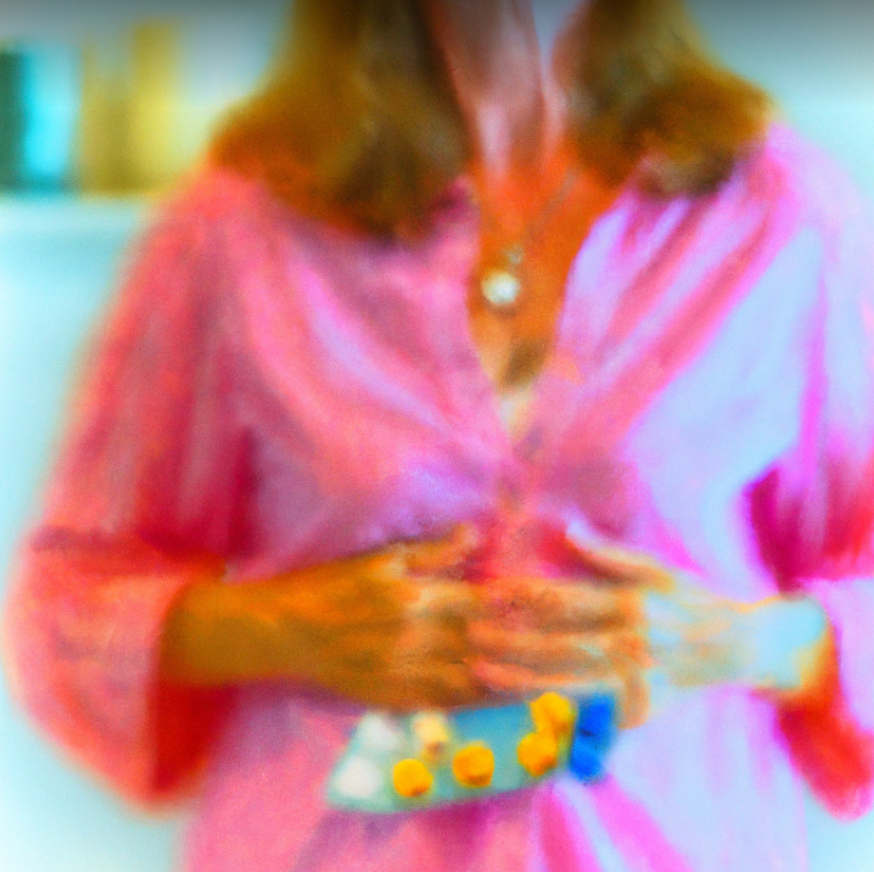
\includegraphics{./graphics/sample_2.png}} &
            \adjustbox{width=4cm,padding=5pt}{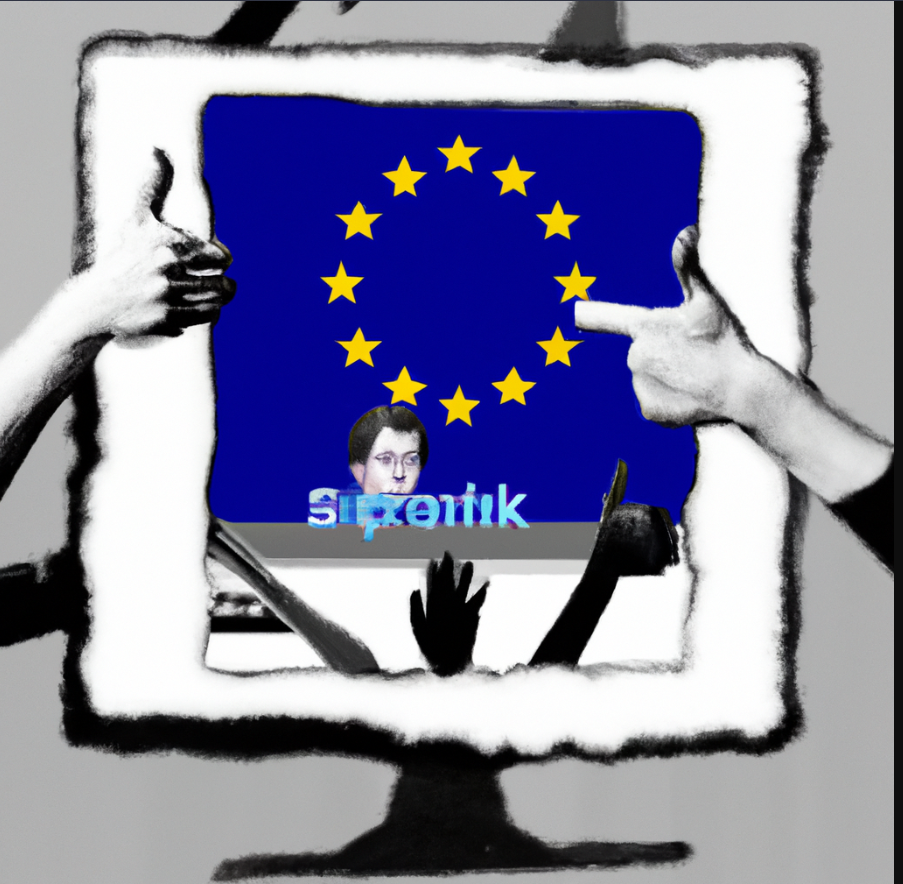
\includegraphics{./graphics/sample_3.png}} \\
            \hline
            Datum & Zaterdag 20 Mei & Zondag 21 Mei & Maandag 22 Mei \\
            \hline
            Gebruikte prompt & "Eenheid voor Oekraïne" in Realistische stijl. &Women's Menopause Symptoms Relieved by Promising New Drug Style: Impressionism. & "Europese Unie geeft Facebook's Meta een recordboete" - Stijl: Surrealisme . \\
            \hline
            Inspiratie & De prompt was gebaseerd op de kernboodschap die ik eerder had gegenereerd op basis van het artikel over Charles Michel en de G7-landen die een langetermijnhulpplan en druk uitoefenden voor Oekraïne. & De kernboodschap die ik heb gegenereerd, is gebaseerd op het artikel "Nieuw medicijn tegen opvliegers op komst: ‘60 tot 70 procent van de vrouwen heeft er last van’", dat in het gegeven JSON-bestand wordt genoemd. & Deze prompt is afgeleid van de belangrijkste titel uit de JSON-gegevens die door de gebruiker zijn verstrekt, met name: "EU geeft Facebook-moederbedrijf Meta recordboete van 1,2 miljard euro". Ik heb de titel verkort tot een gepaste lengte. \\
            \hline
        \end{tabular}
        \caption{Gebruikte samples binnen de turingtest.}
        \label{table:samples}
    \end{table}
\pagebreak

\section{Resultaat}
\label{section:result}
Binnen deze sectie zullen we het resultaat van de turingtest bespreken. We zullen één voor één de persona overlopen en hun bevindingen kort toelichten. We zullen elke test starten met hen te bevragen welke boodschap verborgen zit in elk schilderij.

\subsection{Persona: Ronan}
Ronan is een creatieve ICT-student die graag game development wil studeren. Hij is een getalenteerde tekenaar, maar hij volgt geen nieuws. Laten we eens kijken naar de bevindingen van Ronan op basis van de samples en ontdekken of hij de boodschap heeft kunnen achterhalen.

\subsubsection{Sample 1}
Bij het bekijken van het schilderij merkt Ronan op: "Dat in het midden is niet echt duidelijk, maar het lijkt erop dat er verschillende landen iets willen doen in Oekraïne." \\

Ronan lijkt de kernboodschap van dit schilderij matig te hebben begrepen. Hij heeft opgemerkt dat er verschillende landen betrokken zijn bij een kwestie in Oekraïne. Hoewel hij niet specifiek weet welk artikel hieraan ten grondslag ligt, heeft hij de basis toch begrepen.  \\

Ronan vertelde me dat als de vlaggen die centraal worden afgebeeld een betekenis hadden, indien hij wist waarvoor de vlaggen stonden kon hij waarschijnlijk de kernboodschap hieruit afleiden. 
 
\subsubsection{Sample 2}
Bij het analyseren van dit schilderij geeft Ronan zijn interpretatie: "Iets met medicatie, een nieuw medicijn en/of anticonceptiemiddel? Wat de vrouw in haar hand houdt, kan misschien een nieuw geneesmiddel zijn dat op de markt is gelanceerd." \\

Ronan heeft de boodschap van dit schilderij opgepikt en vermoedt dat het gaat over medicatie. Hij suggereert dat er mogelijk een nieuw medicijn of anticonceptiemiddel is ontwikkeld, en de vrouw in het schilderij houdt misschien het nieuwe geneesmiddel vast. Hoewel hij niet precies weet welk artikel hieraan gerelateerd is, heeft hij een algemeen begrip van het onderwerp. \\
  
\subsubsection{Sample 3}
"Ik zie iets met Europa, een duim omhoog wat duidt op goedkeuring. Het lijkt op een computerscherm, dus misschien heeft het iets te maken met een website. Ik denk dat het Europees Parlement een nieuwe wet heeft goedgekeurd die te maken heeft met regels op het internet." \\

Ronan heeft de boodschap niet kunnen achterhalen. Hij heeft wel opgemerkt dat de EU duidelijk aanwezig is in het schilderij, maar hij herkende de duimpjes niet als de iconische "likes" op Facebook. Na het tonen van het artikel zei Ronan dat het mogelijk was geweest om dit te herkennen, maar dat abstractie correct geïnterpreteerd moet kunnen worden.
 
 
 \subsection{Persona: Arthur}
Arthur is een laatstejaarsstudent Informatica met een matige kennis van kunst. Hoewel hij zelf niet actief betrokken is bij het creëren van kunst, heeft hij een goed begrip van het onderwerp. Arthur volgt het nieuws niet. 
 
 \subsubsection{Sample 1}
Arthur merkte het volgende op: ``Dit gaat gegarandeerd over Oekraïne. Het lijkt erop aan de hand van de vlag dat een groep landen samenwerken binnen Oekraïne voor één bepaald doel.'' \\
 
 We besluiten dat arthur de boodschap van dit schilderij goed begrepen heeft en concludeert dat het gaat over samenwerking tussen landen in Oekraïne. Hoewel hij niet specifiek weet welk artikel hieraan gerelateerd is, heeft hij de essentie begrepen. 
 
 \subsubsection{Sample 2}
 Arthur merkte het volgende op: "Op het eerste gezicht lijkt het alsof een vrouw in dit schilderij lijdt. Ik zie ook medicatie op de tafel liggen. Zou dit kunnen gaan over de nieuwe medicatie voor vrouwen die in hun menopauze zitten?" \\
 
 Arthur heeft de boodschap van dit schilderij opgepikt en vermoedt dat het te maken heeft met het lijden van vrouwen. Hij maakt de associatie met medicatie en suggereert dat het mogelijk gaat over nieuwe medicatie voor vrouwen in hun menopauze. 
 
 \subsubsection{Sample 3}
Arthur had de volgende interpretatie: ``Iets met europese unie, iets dat goedgekeurd moet worden of al is gebeurd?'' \\

Arthur heeft de boodschap van dit schilderij niet specifiek kunnen achterhalen, maar hij herkent de aanwezigheid van de Europese Unie. Hij vermoedt dat het schilderij mogelijk te maken heeft met goedkeuring van iets, ofwel iets dat nog moet gebeuren of al heeft plaatsgevonden. Doordat hij geen specifieke details of context kan geven, heeft hij de boodschap niet kunnen achterhalen. 


\subsection{Persona: Arjan}
Arjan is geboren in Turkije en opgegroeid in Nederland. In zijn jongere jaren heeft hij zich veel beziggehouden met het ontwerpen van logo's en banners voor profielen, wat zijn vaardigheden op het gebied van grafisch ontwerp versterkt. Dit maakt hem een interessante testpersona voor de turingtest, aangezien zijn ervaring en kennis een waardevolle troef kunnen zijn. Arjan volgt enkel de hoogtepunten.
 \subsubsection{Sample 1}
``Ik kan dit artikel niet helemaal plaatsen. Hoewel het over Oekraïne gaat, kan ik de boodschap er niet uit halen. Als ik zou moeten gokken, zou ik zeggen dat er meerdere landen bij betrokken zijn vanwege de aanwezigheid van vlaggen. Maar ik kan de precieze boodschap niet achterhalen.'' \\

Net als de vorige persona kan Arjan ook concluderen dat het artikel over Oekraïne gaat en dat andere landen mogelijk betrokken zijn. De boodschap blijft echter onduidelijk.

\subsubsection{Sample 2}
Arjan vermoedde dat dit kunstwerk ging over een vrouw die verslaafd is aan medicatie. Echter, toen ik hem vertelde dat het eigenlijk ging over een nieuwe medicatie, kon hij meteen zeggen dat het specifiek ging over medicatie voor de menopauze. \\

De oorspronkelijke boodschap werd dus verkeerd geïnterpreteerd door Arjan. Echter, met een hint kon hij wel de juiste boodschap interpreteren.

\subsubsection{Sample 3}
"Europese Unie, televisie, duimen. Heeft dit misschien iets te maken met Facebook? Gaat dit over de boete die de Europese Unie heeft opgelegd aan Meta?"

Arjan heeft de mogelijke connectie gelegd tussen de Europese Unie, televisie en duimen, en vermoedt dat het mogelijk verband houdt met Facebook. Hij suggereert dat het specifiek zou kunnen gaan over de boete die de Europese Unie heeft opgelegd aan Meta. \\

Arjan heeft successvol de boodschap hieruit gehaald en ook de correcte artikel hieraan gelinkt. 


\subsection{Persona: Lucas}
Lucas is een gepassioneerde software engineer die in zijn vrije tijd graag muziek draait. Hoewel hij geen specifieke artistieke achtergrond heeft, is hij wel creatief in zijn vakgebied. Lucas volgt echter het nieuws niet.
\subsubsection{Sample 1}
Bij het bekijken van het schilderij herkende Lucas een gevoel van patriotisme en merkte hij op dat de rode lijn in Oekraïne mogelijk een splitsing of een grens vertegenwoordigde. Hij kon echter geen verband leggen tussen de vlaggen en meerdere landen. Met andere woorden, Lucas kon de exacte boodschap van dit schilderij niet achterhalen.
\subsubsection{Sample 2}
Het wazige beeld en de afbeelding van medicatie deden Lucas denken aan een verslaving. Toen ik hem vertelde dat het schilderij eigenlijk ging over een nieuw medicijn voor vrouwen, kon Lucas de link leggen en begrijpen waar het over ging.
\subsubsection{Sample 3}
Lucas interpreteerde dit schilderij als iets waarover gestemd moest worden. De mensen die hun duim omhoog staken, suggereerden dat er een nieuwe regel of wet werd beoordeeld. Nadat ik hem vertelde dat de duimen eigenlijk het Facebook-symbool waren, kon hij de link leggen, maar slaagde hij er nog steeds niet in om de exacte boodschap eruit te halen.


 \subsection{Persona: Shauny}
Shauny is een laatstejaarsstudente Journalistiek aan de Arteveldehogeschool met een grote interesse in politiek. Shauny volgt bijna dagelijks het nieuws en lijkt me een perfecte persona voor deze turingtest.
 \subsubsection{Sample 1}
 TODO
 \subsubsection{Sample 2}
 TODO
 \subsubsection{Sample 3}
 TODO
\subsection{Persona: Filip}
 TODO
\subsubsection{Sample 1}
 TODO
\subsubsection{Sample 2}
 TODO
\subsubsection{Sample 3}
 TODO
 
\subsection{Persona: Marta}
  TODO
\subsubsection{Sample 1}
TODO
\subsubsection{Sample 2}
TODO
\subsubsection{Sample 3}
 TODO
 
\subsection{Persona: Manu}
  TODO
\subsubsection{Sample 1}
 TODO
\subsubsection{Sample 2}
 TODO
\subsubsection{Sample 3}
 TODO
 
 
 
 % Meer persona's hier ... 
 
 
\section{Meer uitleg}
Het resultaat verkregen van GPT en DALL-E is gebaseerd op patronen en informatie die het model heeft geleerd uit de gegevens waarop het is getraind. Hoewel deze modellen goede prestaties kunnen leveren, zijn er enkele beperkingen waardoor hun output niet altijd 100\% overeenkomt met de realiteit. \\

Ten eerste kan GPT soms de context of intentie van de invoer verkeerd begrijpen of verkeerd interpreteren. Dit kan leiden tot onjuiste of ongepaste antwoorden. Het model kan gevoelig zijn voor subtiele veranderingen in de formulering van de vraag en kan daardoor onverwachte resultaten produceren. \\

Ten tweede kan DALL-E, als een generatief model voor beeldcreatie, soms afbeeldingen genereren die niet volledig relevant zijn voor het huidige nieuws of specifieke vereisten. Hoewel het model in staat is om nieuwe, unieke afbeeldingen te maken op basis van de gegeven prompt, is het niet altijd in staat om contextuele nuances of specifieke details van de gewenste afbeelding te begrijpen. \\

We kunnen besluiten uit de werking van de applicatie dat doordat er nooit eenzelfde uitkomst is en deze uitkomst kan variëren in relevantie tot het nieuws, dat er steeds menselijke controle moet zijn op de foto vooraleer deze kan gebruikt worden binnen bijvoorbeeld een krant die dagelijks een kunstwerk genereert op basis van de artikels die hierin voorkomen. 

 \section{Samengevat}